\section{Time Escape algoritmy}\label{sec:tea}

Pokud se čtenář dostal až do této části, mohl si všimnout, že jednu kategorii fraktálů jsme zatím zcela vynechali. Přitom právě ta je z velké části zodpovědná za popularitu, které se těší toto odvětví matematiky, zejména \emph{Mandelbrotova množina}\index{Mandebrotova množina}\index{množina!Mandebrotova} (viz obrázek \ref{fig:mandebrotova-mnozina}) pojmenovaná po samotném zakladateli fraktální geometrie.
\begin{figure}[h]
    \centering
    
\includegraphics[width=\textwidth]{ch01-mandelbrotova-mnozina.jpg}
    \caption[Mandebrotova množina]{Mandebrotova množina (Převzato z Wikipedia Commons)\footnotemark}
    \label{fig:mandebrotova-mnozina}
\end{figure}
Tím spíš s faktem, že její definice není v konečném důsledku nikterak složitá\footnotetext{Dostupné z \url{https://en.wikipedia.org/wiki/Mandelbrot\_set\#/media/File:Mandel\_zoom\_00\_mandelbrot\_set.jpg}}.

S pravděpodobně nejznámějším fraktálem však souvisí dvojice širších termínů, se kterým začneme, a jsou jimi tzv. \emph{Juliovy množiny}\index{Fatouova množina}\index{množina!Fatouova} a \emph{Fatouovy množiny}\index{Fatouova množina}\index{množina!Fatouova} pojmenované po francouzských matematicích \name{Gastonovi Juliovi} (1893--1978) a \name{Pierre Fatouovi} (1878--1929). Pro jejich studium se však budeme muset ponořit do světa komplexních čísel.

Lze nejspíše předpokládat, že se čtenář nejspíše s komplexními čísly již setkal. Nebudeme se tedy společně hlouběji zabývat naprostými základy. Pouze si stručně připomeňme značení.
\begin{itemize}
    \item \emph{Komplexním číslem}\index{komplexní číslo} rozumíme číslo $z=a+b\imag$, kde $a,b\in\R$ a $\imag^2=-1$. Množinu komplexních čísel, jak už je zvykem, budeme značit $\C$.
    \item \emph{Komplexně sdruženým číslem}\index{Komplexně sdružerné číslo} k číslu $z=a+b\imag$ rozumíme číslo
    \[\cconjugate{z}=a-b\imag.\]
    \item \emph{Absolutní hodnotou komplexního čísla} $z=a+b\imag$ rozumíme vzdálenost od počátku, tj. budeme-li uvažovat metrický prostor $(\C,\varrho)$, pak
    \[|z|=\varrho(z,0).\]
    Nejčastěji však budeme uvažovat eukleidovskou metriku $\varrho_e$, tedy
    \[|z|=\sqrt{a^2+b^2}.\]
\end{itemize}
V této sekci budeme především pracovat s komplexními polynomiálními funkcemi $\mapping{f}{\C}{\C}$, tzn. funkcemi ve tvaru
\[f(z)=\sum_{i=1}^{n}a_iz^i=a_nz^n+a_{n-1}z^{n-1}+\dots+a_1z+a_0.\]
Brzy uvidíme jejich důležitou roli.

\subsection{Juliovy a Fatouovy množiny}\label{subsec:juliovy-fatouovy-mnoziny}

Jak zde již bylo řečeno, exsencí této kapitoly bude práce s tzv. \emph{Juliovými a Fatouovými množinami}\index{Juliova množina}\index{množina!Juliova}\index{Fatouova množina}\index{množina!Fatouova}. Pojďme se tedy podívat, o co se jedná. Ještě připomeňme značení, které jsme zavedli již v části \ref{subsec:hausdorffuv-mp-kontrakce} věnující se IFS na Hausdorffově metrickém prostoru, týkající se skládání funkcí. Obecně $n$-tou iteraci funkce $\mapping{f}{\C}{\C}$ budeme značit
\[f^{\circ n}(z)=(f\circ f^{\circ(n-1)})(z)=f(f(z))\]
kde $z\in\C$.
\begin{definition}[Juliova a Fatouova množina]\label{juliova-fatouova-mnozina}
    Mějme polynomiálními funkci $\mapping{f}{\C}{\C}$. Pak definujeme
    \begin{enumerate}[label=(\alph*)]
        \item \emph{vyplněnou Juliovu množinu}\index{množina!vyplněná Juliova}\index{vyplněná Juliova množina} polynomiální funkce $f$
        \[\filledinjulia(f)=\set{z\in\C\mid f^{\circ n}(z)\notto\infty}.\]
        \item \emph{Juliovu množinu}\index{Juliova množina}\index{množina!Juliova} polynomiální funkce $f$
        \[\julia(f)=\boundary{\filledinjulia(f)}.\]
        \item \emph{Fatouovu množinu}\index{Fatouova množina}\index{množina!Fatouova} polynomiální funkce $f$
        \[\fatou(f)=\C\setminus\julia(f).\]
    \end{enumerate}
\end{definition}
Co nám definice \ref{juliova-fatouova-mnozina} vlastně říká? U pevně zadané funkce $f(z)=\sum_{i=1}^{n}a_iz^i$ pro zadaný bod $z\in\C$ zkoumáme, zda je posloupnost\footnote{Poznamenejme, že limitu posloupnosti komplexní čísel zde chápeme (stejně jako v ostatních případech) jako limitu posloupnosti v metrickém prostoru, jmenovitě $(\C,\varrho_e)$.} jejích postupných iterací $\set{f^{\circ n}(z)}_{n=1}^\infty$ omezená. Později uvidíme, že Juliova množina má v typickém případě charakter fraktálu.
\begin{example}
    \begin{itemize}
        \item Uvažujme identitu $f(z)=z^k$. Pak pro její $n$-tou iteraci platí $f^{\circ n}(z)=z^{k^n}$. Tedy
        \[\filledinjulia(f)=\filledinjulia(\id)=\set{z\in\C\mid |z|<1},\]
        resp.
        \[\julia(f)=\set{z\in\C\mid|z|=1}.\]
        Juliova množina funkce $f$ tvoříjednotkovou kružnici umístěnou v počátku, resp. Juliova množina $J(f)$ tvoří jednotkový kruh.
        \item Pro $f(z)=z^2+c$, kde $c\in\C$ je varianta množiny $K(f)$ znázorněna na obrázku \ref{subfig:juliova-mnozina-1}.
        \item Ještě jiný příklad pro složitější polynom $f(z)=z^3-z^2$ lze vidět na obrázku \ref{subfig:juliova-mnozina-2}.
    \end{itemize}
\end{example}
\begin{figure}[h]
    \centering
    \begin{subfigure}{0.45\textwidth}
        \centering
        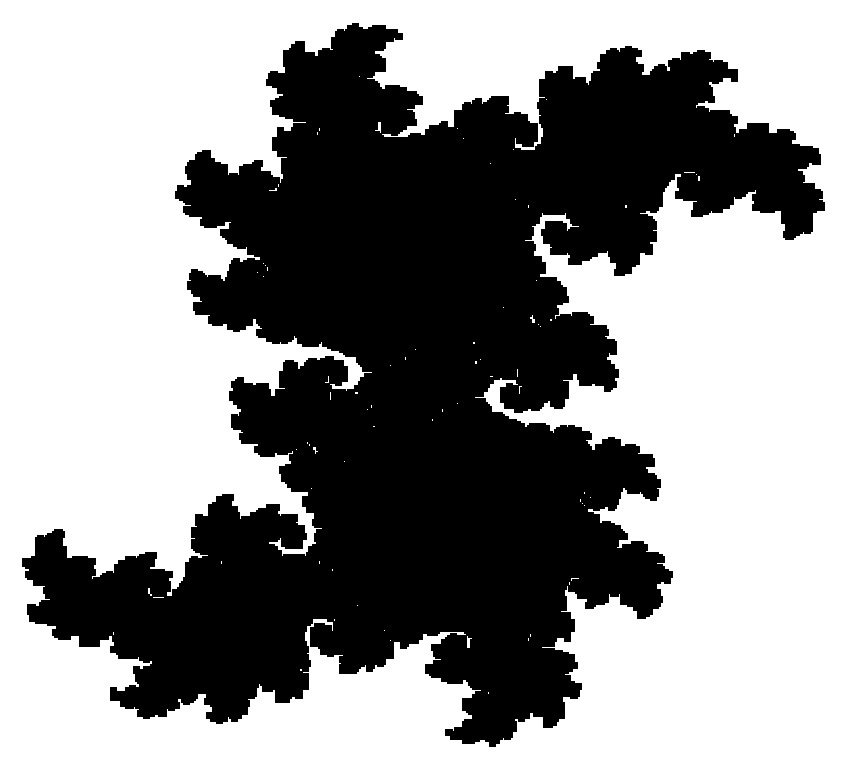
\includegraphics[width=\textwidth]{julia-set-1.pdf}
        \caption{$f(z)=z^2+0.35 + 0.35\imag$}
        \label{subfig:juliova-mnozina-1}
    \end{subfigure}
    \qquad
    \begin{subfigure}{0.45\textwidth}
        \centering
        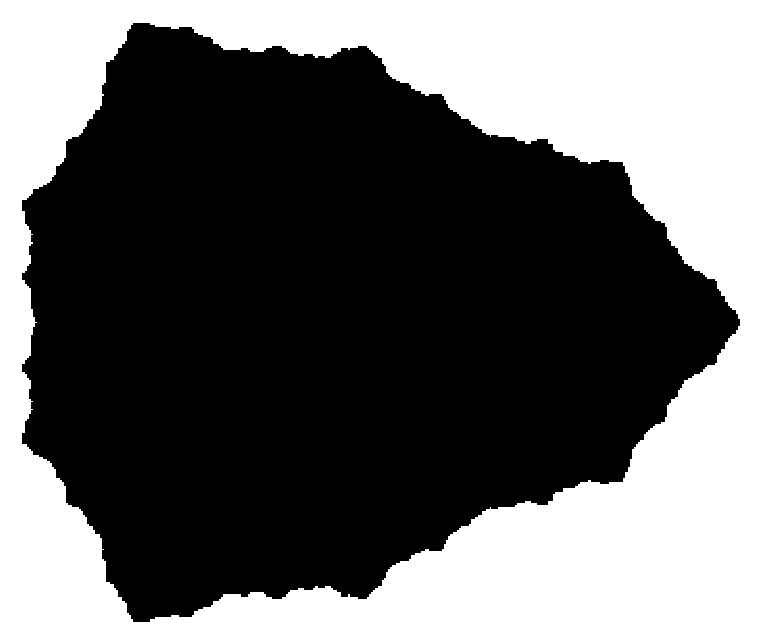
\includegraphics[width=\textwidth]{julia-set-2.pdf}
        \caption{$f(z)=z^3+z^2$}
        \label{subfig:juliova-mnozina-2}
    \end{subfigure}
    \caption{Příklady aproximace $F(f)$}
    \label{fig:priklady-juliovych-mnozin}
\end{figure}